% Generated by Sphinx.
\def\sphinxdocclass{report}
\documentclass[letterpaper,10pt,english]{sphinxmanual}
\usepackage[utf8]{inputenc}
\DeclareUnicodeCharacter{00A0}{\nobreakspace}
\usepackage[T1]{fontenc}
\usepackage{babel}
\usepackage{times}
\usepackage[Bjarne]{fncychap}
\usepackage{longtable}
\usepackage{sphinx}
\usepackage{multirow}


\title{PAPI Documentation}
\date{December 14, 2011}
\release{1.0.1}
\author{J.M.Ibanez (IAA-CSIC)}
\newcommand{\sphinxlogo}{}
\renewcommand{\releasename}{Release}
\makeindex

\makeatletter
\def\PYG@reset{\let\PYG@it=\relax \let\PYG@bf=\relax%
    \let\PYG@ul=\relax \let\PYG@tc=\relax%
    \let\PYG@bc=\relax \let\PYG@ff=\relax}
\def\PYG@tok#1{\csname PYG@tok@#1\endcsname}
\def\PYG@toks#1+{\ifx\relax#1\empty\else%
    \PYG@tok{#1}\expandafter\PYG@toks\fi}
\def\PYG@do#1{\PYG@bc{\PYG@tc{\PYG@ul{%
    \PYG@it{\PYG@bf{\PYG@ff{#1}}}}}}}
\def\PYG#1#2{\PYG@reset\PYG@toks#1+\relax+\PYG@do{#2}}

\def\PYG@tok@gd{\def\PYG@tc##1{\textcolor[rgb]{0.63,0.00,0.00}{##1}}}
\def\PYG@tok@gu{\let\PYG@bf=\textbf\def\PYG@tc##1{\textcolor[rgb]{0.50,0.00,0.50}{##1}}}
\def\PYG@tok@gt{\def\PYG@tc##1{\textcolor[rgb]{0.00,0.25,0.82}{##1}}}
\def\PYG@tok@gs{\let\PYG@bf=\textbf}
\def\PYG@tok@gr{\def\PYG@tc##1{\textcolor[rgb]{1.00,0.00,0.00}{##1}}}
\def\PYG@tok@cm{\let\PYG@it=\textit\def\PYG@tc##1{\textcolor[rgb]{0.25,0.50,0.56}{##1}}}
\def\PYG@tok@vg{\def\PYG@tc##1{\textcolor[rgb]{0.73,0.38,0.84}{##1}}}
\def\PYG@tok@m{\def\PYG@tc##1{\textcolor[rgb]{0.13,0.50,0.31}{##1}}}
\def\PYG@tok@mh{\def\PYG@tc##1{\textcolor[rgb]{0.13,0.50,0.31}{##1}}}
\def\PYG@tok@cs{\def\PYG@tc##1{\textcolor[rgb]{0.25,0.50,0.56}{##1}}\def\PYG@bc##1{\colorbox[rgb]{1.00,0.94,0.94}{##1}}}
\def\PYG@tok@ge{\let\PYG@it=\textit}
\def\PYG@tok@vc{\def\PYG@tc##1{\textcolor[rgb]{0.73,0.38,0.84}{##1}}}
\def\PYG@tok@il{\def\PYG@tc##1{\textcolor[rgb]{0.13,0.50,0.31}{##1}}}
\def\PYG@tok@go{\def\PYG@tc##1{\textcolor[rgb]{0.19,0.19,0.19}{##1}}}
\def\PYG@tok@cp{\def\PYG@tc##1{\textcolor[rgb]{0.00,0.44,0.13}{##1}}}
\def\PYG@tok@gi{\def\PYG@tc##1{\textcolor[rgb]{0.00,0.63,0.00}{##1}}}
\def\PYG@tok@gh{\let\PYG@bf=\textbf\def\PYG@tc##1{\textcolor[rgb]{0.00,0.00,0.50}{##1}}}
\def\PYG@tok@ni{\let\PYG@bf=\textbf\def\PYG@tc##1{\textcolor[rgb]{0.84,0.33,0.22}{##1}}}
\def\PYG@tok@nl{\let\PYG@bf=\textbf\def\PYG@tc##1{\textcolor[rgb]{0.00,0.13,0.44}{##1}}}
\def\PYG@tok@nn{\let\PYG@bf=\textbf\def\PYG@tc##1{\textcolor[rgb]{0.05,0.52,0.71}{##1}}}
\def\PYG@tok@no{\def\PYG@tc##1{\textcolor[rgb]{0.38,0.68,0.84}{##1}}}
\def\PYG@tok@na{\def\PYG@tc##1{\textcolor[rgb]{0.25,0.44,0.63}{##1}}}
\def\PYG@tok@nb{\def\PYG@tc##1{\textcolor[rgb]{0.00,0.44,0.13}{##1}}}
\def\PYG@tok@nc{\let\PYG@bf=\textbf\def\PYG@tc##1{\textcolor[rgb]{0.05,0.52,0.71}{##1}}}
\def\PYG@tok@nd{\let\PYG@bf=\textbf\def\PYG@tc##1{\textcolor[rgb]{0.33,0.33,0.33}{##1}}}
\def\PYG@tok@ne{\def\PYG@tc##1{\textcolor[rgb]{0.00,0.44,0.13}{##1}}}
\def\PYG@tok@nf{\def\PYG@tc##1{\textcolor[rgb]{0.02,0.16,0.49}{##1}}}
\def\PYG@tok@si{\let\PYG@it=\textit\def\PYG@tc##1{\textcolor[rgb]{0.44,0.63,0.82}{##1}}}
\def\PYG@tok@s2{\def\PYG@tc##1{\textcolor[rgb]{0.25,0.44,0.63}{##1}}}
\def\PYG@tok@vi{\def\PYG@tc##1{\textcolor[rgb]{0.73,0.38,0.84}{##1}}}
\def\PYG@tok@nt{\let\PYG@bf=\textbf\def\PYG@tc##1{\textcolor[rgb]{0.02,0.16,0.45}{##1}}}
\def\PYG@tok@nv{\def\PYG@tc##1{\textcolor[rgb]{0.73,0.38,0.84}{##1}}}
\def\PYG@tok@s1{\def\PYG@tc##1{\textcolor[rgb]{0.25,0.44,0.63}{##1}}}
\def\PYG@tok@gp{\let\PYG@bf=\textbf\def\PYG@tc##1{\textcolor[rgb]{0.78,0.36,0.04}{##1}}}
\def\PYG@tok@sh{\def\PYG@tc##1{\textcolor[rgb]{0.25,0.44,0.63}{##1}}}
\def\PYG@tok@ow{\let\PYG@bf=\textbf\def\PYG@tc##1{\textcolor[rgb]{0.00,0.44,0.13}{##1}}}
\def\PYG@tok@sx{\def\PYG@tc##1{\textcolor[rgb]{0.78,0.36,0.04}{##1}}}
\def\PYG@tok@bp{\def\PYG@tc##1{\textcolor[rgb]{0.00,0.44,0.13}{##1}}}
\def\PYG@tok@c1{\let\PYG@it=\textit\def\PYG@tc##1{\textcolor[rgb]{0.25,0.50,0.56}{##1}}}
\def\PYG@tok@kc{\let\PYG@bf=\textbf\def\PYG@tc##1{\textcolor[rgb]{0.00,0.44,0.13}{##1}}}
\def\PYG@tok@c{\let\PYG@it=\textit\def\PYG@tc##1{\textcolor[rgb]{0.25,0.50,0.56}{##1}}}
\def\PYG@tok@mf{\def\PYG@tc##1{\textcolor[rgb]{0.13,0.50,0.31}{##1}}}
\def\PYG@tok@err{\def\PYG@bc##1{\fcolorbox[rgb]{1.00,0.00,0.00}{1,1,1}{##1}}}
\def\PYG@tok@kd{\let\PYG@bf=\textbf\def\PYG@tc##1{\textcolor[rgb]{0.00,0.44,0.13}{##1}}}
\def\PYG@tok@ss{\def\PYG@tc##1{\textcolor[rgb]{0.32,0.47,0.09}{##1}}}
\def\PYG@tok@sr{\def\PYG@tc##1{\textcolor[rgb]{0.14,0.33,0.53}{##1}}}
\def\PYG@tok@mo{\def\PYG@tc##1{\textcolor[rgb]{0.13,0.50,0.31}{##1}}}
\def\PYG@tok@mi{\def\PYG@tc##1{\textcolor[rgb]{0.13,0.50,0.31}{##1}}}
\def\PYG@tok@kn{\let\PYG@bf=\textbf\def\PYG@tc##1{\textcolor[rgb]{0.00,0.44,0.13}{##1}}}
\def\PYG@tok@o{\def\PYG@tc##1{\textcolor[rgb]{0.40,0.40,0.40}{##1}}}
\def\PYG@tok@kr{\let\PYG@bf=\textbf\def\PYG@tc##1{\textcolor[rgb]{0.00,0.44,0.13}{##1}}}
\def\PYG@tok@s{\def\PYG@tc##1{\textcolor[rgb]{0.25,0.44,0.63}{##1}}}
\def\PYG@tok@kp{\def\PYG@tc##1{\textcolor[rgb]{0.00,0.44,0.13}{##1}}}
\def\PYG@tok@w{\def\PYG@tc##1{\textcolor[rgb]{0.73,0.73,0.73}{##1}}}
\def\PYG@tok@kt{\def\PYG@tc##1{\textcolor[rgb]{0.56,0.13,0.00}{##1}}}
\def\PYG@tok@sc{\def\PYG@tc##1{\textcolor[rgb]{0.25,0.44,0.63}{##1}}}
\def\PYG@tok@sb{\def\PYG@tc##1{\textcolor[rgb]{0.25,0.44,0.63}{##1}}}
\def\PYG@tok@k{\let\PYG@bf=\textbf\def\PYG@tc##1{\textcolor[rgb]{0.00,0.44,0.13}{##1}}}
\def\PYG@tok@se{\let\PYG@bf=\textbf\def\PYG@tc##1{\textcolor[rgb]{0.25,0.44,0.63}{##1}}}
\def\PYG@tok@sd{\let\PYG@it=\textit\def\PYG@tc##1{\textcolor[rgb]{0.25,0.44,0.63}{##1}}}

\def\PYGZbs{\char`\\}
\def\PYGZus{\char`\_}
\def\PYGZob{\char`\{}
\def\PYGZcb{\char`\}}
\def\PYGZca{\char`\^}
\def\PYGZsh{\char`\#}
\def\PYGZpc{\char`\%}
\def\PYGZdl{\char`\$}
\def\PYGZti{\char`\~}
% for compatibility with earlier versions
\def\PYGZat{@}
\def\PYGZlb{[}
\def\PYGZrb{]}
\makeatother

\begin{document}

\maketitle
\tableofcontents
\phantomsection\label{index::doc}


{\hfill
\includegraphics{logo_PANIC.jpg}\hfill}

Contents:


\chapter{Introduction}
\label{intro:introduction}\label{intro:welcome-to-papi-s-documentation}\label{intro::doc}
PAPI is an automatic image processing pipeline for data taken with the
PAnoramic Near Infrared Camera (PANIC) on the 2.2m Telescope at Calar Alto Observatory. The pipeline
currently supports imaging data from camera and is written in Python
and C making it portable across many platforms. The automated processing
steps include basic calibration (removeing instrumental signature), cosmic-ray
removal, treatment for post-SAA cosmic ray persistence and electronic ghosts,
sky subtraction, non-linear count-rate correction,
artifact masking, robust alignment and registration for large mosaics,
weight map generation, and drizzling onto a final image mosaic.

\textbf{Development Team:} Jose M. Ibanez (IAA-CSIC)


\section{Caveats}
\label{intro:caveats}
Currently it is only possible for PANIC to reduce data taken with the
Observing Tool (OT), but not manually with GEIRS.
PAPI was primarily developed and optimized for reducing broad-band imaging data of
extragalactic sources (such as imaging data taken for field galaxy surveys and galaxy cluster surveys).
Other types imaging data have been reduced with PAPI but YMMV (See \emph{troubleshooting} for tips).
PAPI is \textbf{not} designed to reduce any kind of field taken with PANIC.

\index{prerequisites}\index{requirements}

\section{Prerequisites}
\label{intro:prerequisites}\label{intro:index-0}
These software must be install for PAPI to run:
\begin{itemize}
\item {} 
\href{http://www.python.org}{python} (2.4 or 2.5)

\item {} 
\href{http://www.sqlite.org}{sqlite} (v3.0 \textgreater{} if using Python 2.4)

\item {} 
\href{http://initd.org/tracker/pysqlite}{pysqlite} (v2.2.0 \textgreater{} if using Python 2.4)

\item {} 
\href{http://www.stsci.edu/resources/software\_hardware/pyraf/stsci\_python}{stsci\_python} (v2.2 \textgreater{})

\item {} 
\href{http://astromatic.iap.fr/software/sextractor/}{SExtractor} (v2.3.2 \textgreater{})

\item {} 
\href{http://hea-www.harvard.edu/RD/ds9}{SAO DS9 and XPA} (if applying user defined masks)

\end{itemize}

\index{installing}\index{building}\index{source}\index{downloading}

\section{Download}
\label{intro:download}\label{intro:index-1}
Download the papi\_latest.tgz file and the papi\_reffiles.tgz file.
\begin{itemize}
\item {} 
\href{http://code.google.com/p/panicdrs/files/papi\_latests.tgz}{papi\_latest.tgz}

\item {} 
\href{http://code.google.com/p/panicdrs/files/papi\_reffiles.tgz}{papi\_reffiles.tgz}

\end{itemize}


\section{Installing}
\label{intro:installing}\begin{enumerate}
\item {} 
Unzip and untar the PAPI files in a suitable location.
\begin{itemize}
\item {} 
tar zxf papi\_X.X.X.tgz

\item {} 
ln -s papi\_X.X.X papi

\item {} 
cd papi

\item {} 
tar zxf papi\_reffiles.tgz

\end{itemize}

\item {} 
Build the source
\begin{itemize}
\item {} 
cd src

\item {} 
make

\item {} 
make install

\end{itemize}

\item {} 
Edit \code{papi\_setup} script
\begin{itemize}
\item {} 
Modify the PAPI\_DIR and PAPI\_PIPE in the papi\_setup.{[}sh{]}{[}.csh{]} file in the PAPI bin directory

\item {} 
Add the papi\_setup.{[}sh{]}{[}.csh{]} to your .bash\_profile or .cshrc (.tcshrc)
\begin{itemize}
\item {} 
Bash: \code{. \$PAPI\_DIR/bin/papi\_setup.sh}

\item {} 
CSH: \code{source \$PAPI\_DIR/bin/papi\_setup.csh}

\end{itemize}

\end{itemize}

\end{enumerate}

Example papi\_setup.sh:

\begin{Verbatim}[commandchars=\\\{\}]
\#------------------------------------------------------------------------------
\# User Configurable Settings
\#------------------------------------------------------------------------------

\# path to PAPI directory
export PAPI\_DIR=\$\PYGZob{}HOME\PYGZcb{}/pipelines/papi

\# path to PAPI output data products
export PAPI\_PIPE=\$\PYGZob{}HOME\PYGZcb{}/Data

\#------------------------------------------------------------------------------
\# Fixed Settings
\#------------------------------------------------------------------------------
\# path to PAPI reference files
export PAPI\_REF=\$\PYGZob{}PAPI\_DIR\PYGZcb{}/PAPI\_REF
export PATH=\$\PYGZob{}PATH\PYGZcb{}:\$\PYGZob{}PAPI\_DIR\PYGZcb{}/bin
export PYTHONPATH=\$\PYGZob{}PYTHONPATH\PYGZcb{}:\$\PYGZob{}PAPI\_DIR\PYGZcb{}/lib
\end{Verbatim}


\chapter{User Guide}
\label{user_guide:user-guide}\label{user_guide::doc}
This will contain instructions for end users of the application.


\chapter{Developer Guide}
\label{developer_guide::doc}\label{developer_guide:developer-guide}
This will contain instructions for developers of the application.


\chapter{Modules}
\label{modules:modules}\label{modules::doc}
The PAPI pipeline includes N processing steps from basic calibration
to generating final co-added registered mosaics (See table below). Among these
steps are steps for successfully handling three of the most common PANIC
anomalies: electronic ghosting, the pedestal effect and cosmic-ray persistence.
Electronic ghosts occur when a bright object is observed in one of the four
quadrants on a PANIC detector. This results in an echo of the bright object
in the other three quadrants. The module undopuft attempts to remove these
artifacts. The pedestal effect is the result of variable biases in each of the four
PANIC quadrants - leaving a significant pedestal signature in the processed
data.

\index{modules}
\begin{tabulary}{\linewidth}{|r|l|}
\hline
\textbf{
Module
} & \textbf{
Description
}\\\hline

\code{papi}
 & 
Ingest uncalibrated data and builds a SQLite database containing fits header data
\\\hline

\code{calDark}
 & 
Removes electronic ghosts (a.k.a. the ``Mr. Staypuft'' effect)
\\\hline

\code{calDarkModel}
 & 
Basic calibration, sky subtraction/pedestal effect removal, cosmic-ray rejection
\\\hline

\code{calBPM}
 & 
Removes cosmic-ray persistence signal if target was observed shortly after the SAA
\\\hline

\code{calDomeFlat}
 & 
Removes residual instrument signatures by subtracting a ``super-median'' reference image
\\\hline

\code{calTwFlat}
 & 
Uses bicubic spline to flatten the background
\\\hline

\code{calSuperFlat}
 & 
Corrects for count-rate non-linearity
\\\hline

\code{calGainMap}
 & 
Apply user-defined masks (optional)
\\\hline

\code{calNonLinearity}
 & 
Uses object matching algorithms to improve image alignment and registration
\\\hline

\code{checkQuality}
 & 
Creates accurate \emph{RMS} maps for use with MultiDrizzle
\\\hline

\code{eval\_focus\_serie}
 & 
Creates final CR-cleaned, distortion-free drizzled image mosaics using multidrizzle
\\\hline

\code{astrowarp}
 & 
Create final aligned and coadded frame using SEx,SCAMP and SWARP
\\\hline
\end{tabulary}


\index{setup}\index{sqlite}

\section{\texttt{papi}}
\label{modules:papi}\label{modules:index-1}
The \code{papi} module in the main PAPI routine that start the data reduction.
It starts by creating a subdirectory in the \code{PAPI\_DIR} using the run name
give on the command line.  Within the run directory the following
subdirectories are created:

\begin{tabulary}{\linewidth}{|r|l|}
\hline
\textbf{
Directory
} & \textbf{
Description
}\\\hline

\code{CALIB}
 & 
A copy of all the uncalibrated input data and the output processed data products for modules \code{undupuft} through \code{nonlincor}
\\\hline

\code{ALIGN}
 & 
Output processed data products for modules \code{weightmap} through \code{mdrizzle}
\\\hline

\code{FINAL}
 & 
The final data products (final image mosiacs, weightmaps and context images)
\\\hline
\end{tabulary}


NICRED creates a \href{http://www.sqlite.org}{SQLite} database to store the uncalibrated input data fits headers and pipeline metadata:

\index{log}\index{logging}\index{status}\index{FITS}\index{headers}
\begin{tabulary}{\linewidth}{|r|l|}
\hline
\textbf{
Table
} & \textbf{
Description
}\\\hline

\code{headers}
 & 
Select FITS header keywords for all input images
\\\hline

\code{run\_log}
 & 
Runtime log messages
\\\hline

\code{run\_pars}
 & 
Value of each runtime option
\\\hline

\code{run\_status}
 & 
Runtime status information for each module
\\\hline

\code{raw}
 & 
A \emph{VIEW} of the header table listing only the raw FITS image headers
\\\hline
\end{tabulary}


\index{undopuft}\index{staypuft}

\section{\texttt{undopuft}}
\label{modules:undopuft}\label{modules:index-3}
The \code{undopuft} module attempts to remove the electronic ghosts that can appear when observing
a bright source. For details see \href{http://www.stsci.edu/hst/nicmos/performance/anomalies/staypuft.html}{Electronic Ghosts: Mr. Staypuft, Ringing, and Streaking}.

\index{calped}\index{calnica}\index{pedsky}\index{cridcalc}\index{multiaccum}\index{calibration}

\section{\texttt{calped}}
\label{modules:index-4}\label{modules:calped}
The \code{calped} module performs basic instrumental calibration (dark current subtraction, flat fielding,
conversion to count rates, and cosmic ray identification and rejection) and attempts to remove
the NICMOS pedestal effect. These task are performed by the STSCI IRAF package tasks \href{http://stsdas.stsci.edu/cgi-bin/gethelp.cgi?calnica}{calnica} and \href{http://stsdas.stsci.edu/cgi-bin/gethelp.cgi?pedsky.hlp}{pedsky}.

The NICMOS pedestal effect is the result of variable biases in each of the four NICMOS detector quadrants these
varying bias levels can leave a significant pedestal signature in the processed data. For details see the
NICMOS anomaly page \href{http://www.stsci.edu/hst/nicmos/performance/anomalies/pedestal.html}{Residual Bias (Pedestal)}

NICRED runs all of the calibration steps provided by \href{http://stsdas.stsci.edu/cgi-bin/gethelp.cgi?calnica}{calnica} in the default sequence with the exception of one
additional step. Before the \href{http://stsdas.stsci.edu/cgi-bin/gethelp.cgi?calnica}{calnica} cosmic ray identification and removal step \emph{CRIDCALC} is run NICRED runs an
additional step to improve the cosmic ray rejection. For NICMOS MultiAccum mode observations, \emph{CRIDCALC} assumes
that accumulating background counts over the entire observation is a linear function. This assumption may not
be the true for all observations. Depending on circumstances of the observation the background
count rate may vary over the duration of the observation. In order to determine if the background count rate
is sufficiently non-linear, NICRED computes the median of the first and last three readouts of the MultiAccum
observation.  If the NIRCED finds the count rate has varied it applies the additional step of running \href{http://stsdas.stsci.edu/cgi-bin/gethelp.cgi?pedsky.hlp}{pedsky}
on each of the individual readouts in the MultiAccum observation. This additional step assures the background
count rate is linear before running the \emph{CRIDCALC} step.

\index{saaclean}\index{SAA}\index{pyraf}

\section{\texttt{saaclean}}
\label{modules:saaclean}\label{modules:index-5}
The \code{saaclean} module removes cosmic ray persistence due to observations following an HST transit of
the South Atlantic Anomaly (SAA). See \href{http://www.stsci.edu/hst/nicmos/documents/isrs/isr\_2007\_001.pdf}{Removing Post-SAA Persistence in NICMOS Data}.
NICRED uses the \href{http://www.stsci.edu/resources/software\_hardware/pyraf}{PyRAF} task \code{saaclean} to perform this processing.


\section{\texttt{medsub}}
\label{modules:medsub}\label{modules:pyraf}
The \code{medsub} module attempts to remove any residual instrument signature left over after basic calibration
by subtracting a ``super-median'' reference image. These super-median images are created by median stacking a large
number of images that have been processed by the NICRED modules \code{undopuft}, \code{calped} and \code{saaclean}.
Many super-median reference images (based on various camera, sample-sequence, observation window or HST proposal ID,
and filter combinations) have been pre-generated and are provided in \href{http://www.firstgalaxies.org/downloads/nicred/nicred\_reffiles.tgz}{nicred\_reffiles.tgz}.

\code{medsub} uses the following criteria for determining which super-median image to use:
\begin{enumerate}
\item {} 
Same camera.

\item {} 
Same sample sequence.

\item {} 
Same filter.

\item {} 
Same HST proposal ID (PROP\_ID fits header keyword). Or..

\item {} 
The super-median reference image with and observation date nearest the observation date of the input image.

\end{enumerate}


\section{\texttt{flatten}}
\label{modules:flatten}
The \code{flatten} module attempts to remove any discontinuities between the four quadrants of a NICMOS camera 2 or 3 image.
Discontinuities between quadrants can occur when an exposure contains a large bright object in one of the quadrants.

\index{nonlincor}\index{non-linearity}\index{count-rate}

\section{\texttt{nonlincor}}
\label{modules:index-6}\label{modules:nonlincor}
The \code{nonlincor} module corrects NICMOS images for their count-rate dependent
non-linearity. It used the header keywords CAMERA and FILTER to determine the
non-linearity parameter. It corrects the first image, and in the case of a
multi-extension image, the second image as well, with the appropriate power law.
For details see \href{http://www.stsci.edu/hst/nicmos/documents/isrs/isr\_2006\_003.pdf}{Correcting the NICMOS count-rate
dependent non-linearity}

\index{mask}\index{masking}\index{applymask}\index{ds9}

\section{\texttt{applymask}}
\label{modules:index-7}\label{modules:applymask}
NICRED has the ability to mask any residual artifacts that may occur in one's
data (e.g., as may occur when satellites pass through the HST focal plane).
Masks are easily generated using \href{http://http://hea-www.harvard.edu/RD/ds9}{SAO’s DS9}
image display tool using the following procedure:
\begin{enumerate}
\item {} 
Display all \code{\_cal4.fits} images in DS9.

\item {} 
Marked artifacts on each image with the DS9 polygon region tool.

\item {} 
A script is run that saves a DS9 region file for each image which has a marked artifact.

\item {} 
A second script is run that applies the marked regions in these region files to the associated image’s data-quality array.

\end{enumerate}

{\hfill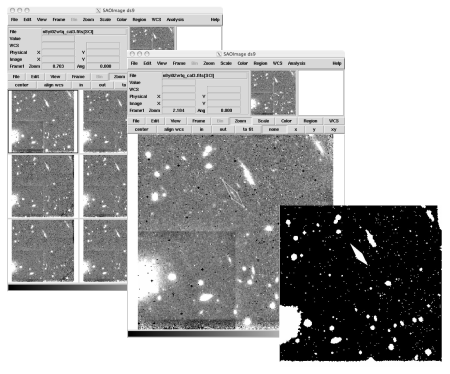
\includegraphics{applymask.png}\hfill}


\section{\texttt{align}}
\label{modules:align}
The \code{align} module uses the external package \code{superalign} to determine the internal
shifts and rotations for an arbitrary number of (overlapping)
contiguous images from a set of (distortion free) catalogs.  It
requires good initial guesses for the shifts and rotations (within 2.5
arcsec and 0.5 degrees of the true solution, respectively), and thus
is ideal for use with NICMOS HST data where these quantities are
approximately known.  It offers several useful advantages relative to
other alignment programs:
\begin{enumerate}
\item {} 
It does not require that all images be contiguous with a single reference image.
This allows one to construct arbitrarily large mosaics out of individual images.

\item {} 
Input catalogs can include substantial (\textgreater{}80\%) contamination from cosmic rays.

\end{enumerate}

For more details on \code{superalign} see the Appendix section \emph{superalign}.

\index{multidrizzle}\index{weightmap}\index{variance}

\section{\texttt{weightmap}}
\label{modules:weightmap}\label{modules:index-8}
The \code{weightmap} module generates an inverse variance weigh map image of each input image as input to MultiDrizzle.

Where \emph{D} is the dark image; \emph{A} is the amplifier glow image; \emph{G} is the gain; \emph{B} is the average background as computed by \code{calnica}; \emph{sigma} is the readnoise; \emph{f} is the inverse flatfield image; and \emph{t} is the exposure time.

\index{multidrizzle}\index{dithering}\index{weightmap}\index{variance}

\section{\texttt{mdrizzle}}
\label{modules:index-9}\label{modules:mdrizzle}
The \code{mdrizzle} module performs cosmic ray rejection and combination of dithered observations using the STSCi software package MultiDrizzle.
For a complete discussion of MultiDrizzle and the Drizzle alorgithm for combining dithered imaging data see the \href{http://incubator.stsci.edu/mediawiki/index.php/Telescopedia:Multidrizzle}{MultiDrizzle Handbook Wiki}.


\chapter{Indices and tables}
\label{index:indices-and-tables}\begin{itemize}
\item {} 
\emph{genindex}

\item {} 
\emph{modindex}

\item {} 
\emph{search}

\end{itemize}



\renewcommand{\indexname}{Index}
\printindex
\end{document}
